\section{Sequences in Euclidean Space} 

  We assume that you know what sequences are, and what it means for them to converge in $\mathbb{R}^n$. Let's primarily focus on sequences in $\mathbb{R}$. Note that there are many way in which a sequence can be divergent. 
  \begin{enumerate}
    \item Increasing/decreasing indefinitely
    \item Oscillating between two constant values
    \item Oscillating between a value tending to $+\infty$ and a value tending to $-\infty$
    \item Many other classes of divergence
  \end{enumerate}

  \begin{definition}[Sequence Tending to Infinity]
    The sequence $\{x_n\}$ \textbf{tends to positive infinity} if for each number $c$ there exists $N \in \mathbb{N}$ such that $x_n > c$ for all $n > N$. It is denoted 
    \begin{equation}
      x_n \rightarrow + \infty \text{ or } \lim_{n \rightarrow \infty} x_n = + \infty
    \end{equation}
    We define sequences that \textbf{tend to negative infinity} similarly. And $\{x_n\}$ \textbf{tends to infinity} if for each $c$ there exists $N \in \mathbb{N}$ such that $|x_n| > c$ for all $n > N$, which is written 
    \begin{equation}
      x_n \rightarrow \infty
    \end{equation}
  \end{definition}

  Note that 
  \begin{equation}
    x_n \rightarrow +\infty \text{ or } x_n \rightarrow -\infty \implies x_n \rightarrow \infty
  \end{equation}
  but the converse is not necessarily true. The simple example is the sequence $x_n = (-1)^n n$. Also, it is important to know that a sequence may be unbounded and yet not tend to $+\infty$, $-\infty$, or $\infty$. 

  \begin{example}[Unbounded Sequence that Doesn't tend to $\infty$]
    The sequence $x_n = n^{(-1)^n}$ is divergent yet does not tend to positive infinity, negative infinity, nor infinity. 
  \end{example} 

  \begin{definition}[Monotonic Sequences]
    Let $X$ be an ordered set. $(x_n)$ is 
    \begin{enumerate}
      \item \textbf{strictly increasing} if $x_{n+1} > x_n$ for all $n$.
      \item \textbf{strictly decreasing} if $x_{n+1} < x_n$ for all $n$.
      \item \textbf{increasing (nondecreasing)} if $x_{n+1} \geq x_n$ for all $n$.
      \item \textbf{decreasing (nonincreasing)} if $x_{n+1} \leq x_n$ for all $n$.
    \end{enumerate}
    Sequences of these types are called \textbf{monotonic}. 
  \end{definition}

  The properties of a general metric space give us some general conditions to determine whether a sequence converges in $\mathbb{R}^n$. To add to our toolbox in determining convergence, we will focus on sufficient conditions for convergence in $\mathbb{R}$, which has the additional properties of being an ordered field. These additional structures unlock a whole new suite of theorems in convergence. Why do we want to focus on just real-valued, i.e. numerical, sequences? First is that since $\mathbb{R}^n$ is constructed as the product topology of $\mathbb{R}$, we can prove a lot about continuity of functions in $\mathbb{R}^n$ by proving limits in $\mathbb{R}$, and letting the construction of the product topology do the rest. Second, the codomain of many natural structures such as inner products, norms, and measures lie in the reals, and we often need to prove convergence of these values.  

\subsection{Convergence Theorems from Completeness and Order}

  So far, in order to show that a sequence is convergent, we must identify a real number first and then show using the $\epsilon$-$\delta$ definition that it converges. This might be overkill in a case where we just want to prove that a sequence converges, but we don't care what it converges to. The following theorems are direct consequences of the Cauchy-completeness and the least upper bound property of the reals. 

  \begin{theorem}[Cauchy-Convergence Criterion]
    A cauchy sequence in $\mathbb{R}$ converges. 
  \end{theorem} 
  \begin{proof}
    This is by definition true, and to see how other forms of completeness implies Cauchy convergence, see above. 
  \end{proof}

  The second result is an immediate consequence of Dedekind completeness, which is equivalent to Cauchy completeness in the reals.  

  \begin{theorem}[Convergence Criterion for Monotonic Sequences]
    \label{thm:monotone-convergence}
    Let $(x_n)_n$ be a sequence. 
    \begin{enumerate}
      \item If $(x_n)$ is monotonically increasing/decreasing and bounded above/below in $\mathbb{R}$, then it converges. 
      \item If $(x_n)$ is monotonically increasing/decreasing in $\mathbb{R} \cup \{\pm \infty\}$, then it converges. 
    \end{enumerate}
  \end{theorem}
  \begin{proof}
    It satisfies to prove the first case, as the second case can be done similarly without much difficulty. Let $x_n \leq x_{n+1}$. Then the set $\{x_n\}$ is bounded above in $\mathbb{R}$, which has the least upper bound property, and so there exists a least upper bound $x$. We claim that the sequence converges to $x$. For every $\epsilon > 0$, since it is least, there exists at least one $x_N \in (x - \epsilon, x)$. By monotonicity, this means that $x_n \in (x - \epsilon, x)$ for all $n \geq N$, and so the sequence converges to $x$. 
  \end{proof}

  We are able to see how both Cauchy and Dedekind completeness of the reals define convergence in $\mathbb{R}$. Now let's squeeze a bit more out of the total ordering to gain some properties of convergence and divergence.   
  
  \begin{theorem}[Preservation of Ordering Between Sequences and Limits]
    Given convergent sequences $(x_n)$ and $(y_n)$, if 
    \begin{equation}
      \lim_{n \rightarrow \infty} x_n < \lim_{n \rightarrow \infty} y_n
    \end{equation}
    then there exists an index $N \in \mathbb{N}$ such that $x_n < y_n$ for all $n > N$. 
  \end{theorem}
  \begin{proof}
    Given $x_n \rightarrow x, y_n \rightarrow y$ and $x < y (\in \mathbb{R})$, then for every $\epsilon > 0$, there exists $N_1, N_2 \in \mathbb{N}$ s.t. $d(x, x_n) < \epsilon$ for all $n > N_1$ and $d(y, y_n) < \epsilon$ for all $n > N_2$. Setting $N = \max\{N_1, N_2\}$, we can say the same for all $n > N$. We choose $\epsilon = \frac{y - x}{2} > 0$. Then, there exists $N \in \mathbb{N}$ s.t. $x_n \in (x - \epsilon, x + \epsilon)$ and $y_n \in (y - \epsilon, y + \epsilon)$ for all $n > N$. Therefore, if $a \in (x - \epsilon, x + \epsilon)$ and $b \in (y - \epsilon, y + \epsilon)$, then 
    \begin{equation}
      a < \sup B_\epsilon (x) = x + \epsilon = y - \epsilon = \inf B_\epsilon (y) < b
    \end{equation}
    which implies that $x_n < y_n$ for all $n > N$. 
  \end{proof}

  \begin{theorem}[Squeeze Theorem for Sequences]
    Given sequences $(x_n), (y_n), (z_n)$ such that 
    \begin{equation}
      x_n \leq y_n \leq z_n
    \end{equation}
    for all $n > N$, if $\{x_n\}$ and $\{z_n\}$ both converge to the same limit, then the sequence $\{y_n\}$ also converges to that limit. That is, 
    \begin{equation}
      \lim_{n \rightarrow \infty} x_n = \lim_{n \rightarrow \infty} z_n = A \implies \lim_{n \rightarrow \infty} y_n = A
    \end{equation}
  \end{theorem} 
  \begin{proof}
    We first prove that if there exists a $N \in \mathbb{N}$ s.t. $a_n \leq b_n$ for all $n > N$, then $\lim_{n \rightarrow \infty} a_n = a \leq b = \lim_{n \rightarrow \infty} b_n$. Assume this weren't true, that $a > b$. Then for $\epsilon = \frac{a - b}{2} > 0$, there must exist $M \in \mathbb{N}$ s.t. $a_n \in (a - \epsilon, a + \epsilon)$ and $b_n \in (b - \epsilon, b + \epsilon)$ for all $n > M$. But 
    \begin{equation}
      b_n < \sup (b - \epsilon, b + \epsilon) = b + \epsilon = a - \epsilon = \inf (a - \epsilon, a + \epsilon) < a_n
    \end{equation}
    which contradicts $a_n \leq b_n$. Therefore, $a \leq b$. Therefore, we can use this to get 
    \begin{equation}
      A = \lim_{n \rightarrow \infty} x_n \leq \lim_{n \rightarrow \infty} y_n \leq \lim_{n \rightarrow \infty} z_n = A \implies \lim_{n \rightarrow \infty} y_n = A
    \end{equation}
  \end{proof}

  \begin{theorem}[Unbounded Sequence has Subsequence Tending to Infinity]
    If $(x_n)$ is not bounded above then it has a subsequence $x_{n_k} \rightarrow +\infty$. 
  \end{theorem}
  \begin{proof}
    We can construct such a subsequence. 
  \end{proof}

  Therefore, we can construct a subsequential limit to $\pm \infty$ if $(x_n)$ is not bounded. If it is bounded, then by the Bolzano-Weierstrass theorem it contains a convergent subsequence. Therefore, we have the following. 

  \begin{corollary}
    \label{existence}
    From each sequence of real numbers there exists either a convergent subsequence or a subsequence tending to infinity. 
  \end{corollary}
  \begin{proof}
    If it's bounded, then Bolzano-Weierstrass. If it's not bounded, then use previous theorem. 
  \end{proof}

  \begin{example}
    We claim that
    \begin{equation}
      \lim_{n\rightarrow \infty} \sqrt[n]{n} = 1
    \end{equation}
  \end{example}

\subsection{Arithmetic}

  \begin{theorem}[Arithmetic on Limits]
    Given that $(x_n), (y_n)$ are numerical sequences with $y_n \neq 0$ for all $n$, and let 
    \begin{equation}
      \lim_{n \rightarrow \infty} x_n = x, \qquad \lim_{n \rightarrow \infty} y_n = y \neq 0
    \end{equation}
    then, 
    \begin{align}
      & \lim_{n\rightarrow \infty} (x_n + y_n) = x + y \\
      & \lim_{n \rightarrow \infty} (c x_n) = c x \\
      & \lim_{n \rightarrow \infty} (x_n \cdot y_n) = x \cdot y \\
      & \lim_{n \rightarrow \infty} \frac{x_n}{y_n} = \frac{x}{y}
    \end{align}
    It immediately follows that the set of all convergent sequences in $\mathbb{R}^\mathbb{N}$ is a subspace of $\mathbb{R}^\mathbb{N}$. 
  \end{theorem}
  \begin{proof}
    For every $\epsilon > 0$, there exists $N_1, N_2 \in \mathbb{N}$ such that
    \begin{align}
      |x_n - x| &< \epsilon \text{ for all } n > N_1 \\
      |y_n - y| &< \epsilon \text{ for all } n > N_2
    \end{align}
    Therefore, for a given $\epsilon$, we wish to prove that there exists a $N$ such that for all $n > N$, 
    \begin{align}
      1. & |(x_n + y_n) - (x+y)| < \epsilon \\
      2. & |c x_n - cx| < \epsilon \\
      3. & |(x_n y_n) - (xy)| < \epsilon \\
      4. & \bigg| \frac{x_n}{y_n} - \frac{x}{y} \bigg| < \epsilon
    \end{align}
    \begin{enumerate}
      \item yy the triangle inequality, we can see that
      \begin{equation}
        |(x_n + y_n) - (x+y)| = |x_n - x| + |y_n - y|
      \end{equation}
      Since we can choose the error between $x_n$ and $x$ for $n > N_1$, and $y_n$ and $y$ for $n>N_2$ as small as we want, we set it to $\epsilon/2$. Then, we have
      \begin{equation}
        |(x_n + y_n) - (x+y)| = |x_n - x| + |y_n - y| < \frac{\epsilon}{2} + \frac{\epsilon}{2} = \epsilon
      \end{equation}
      for all $n> N = \max\{N_1, N_2\}$. Therefore, for a given $\epsilon$, there exists an $N$ such that 
      \begin{equation}
        |(x_n + y_n) - (x+y)| < \epsilon \text{ for all } n > N
      \end{equation}
      \item This proof is easy. For a given $\epsilon$, we choose the error to be $\frac{\epsilon}{c}$.
      \begin{equation}
        |x_n - x| < \frac{\epsilon}{c} \text{ for all } n >N_1
      \end{equation}
      Then, there exists natural number $N_1$ such that
      \begin{equation}
        |c x_n - c x| < c |x_n - x| =  c \frac{\epsilon}{c} = \epsilon \text{ for all } n > N_1
      \end{equation}
      \item We first observe that since the limit of $\{y_n\}$ exists, it must be bounded by a value, say $y$. That is, 
      \begin{equation}
        |y_n| < Y \text{ for all } n \in \mathbb{N}
      \end{equation}
      Then, we see that
      \begin{align}
        |x_n y_n - xy| & = |(x_n y_n - xy_n) + (xy_n - xy)| \\
        & < |x_n y_n - x y_n| + |x y_n - xy| \\
        & = |y_n| |x_n - x| + |x| |y_n - y|
      \end{align}
      Suppose $\epsilon > 0$ is given. Then, we can set the error bounds freely; there exists $N_1, N_2 \in \mathbb{N}$ such that 
      \begin{align}
        |x_n - x| < \frac{\epsilon}{2Y} \text{ for all } n > N_1 \\
        |y_n - y| < \frac{\epsilon}{2|x|} \text{ for all } n > N_2
      \end{align}
      Then, we can see that 
      \begin{equation}
        |x_n y_n - xy| \leq |y_n||x_n -x| + |x| |y_n - y| < Y \cdot \frac{\epsilon}{2Y} + |x| \frac{\epsilon}{2|x|} = \epsilon
      \end{equation}
      for all $n> N = \max\{N_1, N_2\}$.

      \item We use the estimate
      \begin{equation}
        \bigg| \frac{x}{y} - \frac{x_n}{y_n} \bigg| = \frac{|x_n| |y_n - y| + |y_n||x_n - x|}{y_n^2} \cdot \frac{1}{1 - \delta(y_n)}, \;\;\; \delta(y_n) = \frac{|y_n - y|}{|y_n|}
      \end{equation}

      For a given $\epsilon > 0$, we find natural numbers $N_1, N_2$ such that 
      \begin{align}
        |x_n - x| & < \min\Big\{ 1, \frac{\epsilon|y|}{8} \Big\} \text{ for all } n > N_1 \\
        |y_n - y| & < \min \Big\{ \frac{|y|}{4}, \frac{\epsilon y^2}{16(|x| + 1)} \Big\} \text{ for all } n > N_2 
      \end{align}
      From this we can deduce that 
      \begin{equation}
        |x_n| = |x_n - x + x| < |x_n - x| + |x| < |x| + 1
      \end{equation}
      and
      \begin{align}
        |y| & = |y_n + y - y_n| < |y_n| + |y - y_n| \\
        \implies & |y_n| > |y| - |y_n - y| > |y| - \frac{|y|}{4} > \frac{|y|}{2} \\
        \implies & \frac{1}{|y_n|} < \frac{2}{|y|} \\
        \implies & 0 < \delta(y_n) = \frac{|y_n - y|}{|y_n|} < \frac{|y|/4}{|y|/2} = \frac{1}{2} \\
        \implies & 1 - \delta(y_n) > \frac{1}{2}\\
        \implies & 0 < \frac{1}{1 - \delta(y_n)} < 2
      \end{align}
      So, we can substitute 
      \begin{align}
        |x_n| \cdot \frac{1}{y_n^2} \cdot |y_n - y| & < (|x| + 1) \cdot \frac{4}{y^2} \cdot \frac{\epsilon \cdot y^2}{16(|x|+1)} = \frac{\epsilon}{4} \\
        \bigg|\frac{1}{y_n} \bigg| \cdot |x_n - x| & < \frac{2}{|y|} \cdot \frac{\epsilon |y|}{8} = \frac{\epsilon}{4} 
      \end{align}
      into the final equation to get
      \begin{equation}
        \bigg| \frac{x}{y} - \frac{x_n}{y_n}\bigg| < \epsilon \text{ for all } n > N= \max\{N_1, N_2\}
      \end{equation}
    \end{enumerate}
  \end{proof}

  \begin{example}
    We claim that 
    \begin{equation}
      \lim_{n\rightarrow \infty} \frac{n}{q^n} = 0 \text{ if } q>1
    \end{equation}
    Since $x_n = \frac{n}{q^n} \implies x_{n+1} = \frac{n+1}{nq} x_n$ for $n \in \mathbb{N}$. Since 
    \begin{equation}
      \lim_{n\rightarrow \infty} \frac{n+1}{nq} = \lim_{n \rightarrow \infty} \bigg(1 + \frac{1}{n}\bigg) \frac{1}{q} = \lim_{n\rightarrow \infty} \bigg( 1 + \frac{1}{n} \bigg) \cdot \lim_{n\rightarrow \infty} \frac{1}{q} = 1 \cdot \frac{1}{q} = \frac{1}{q} < 1
    \end{equation}
    there exists an index $N$ such that $\frac{n+1}{nq} < 1$ for $n>N$. Thus, we have 
    \begin{equation}
      x_n > x_{n+1} = x_n \cdot \frac{n+1}{nq} \text{ for } n > N
    \end{equation}
    which means that the sequence will be monotonically decreasing from index $N$ on. The terms of the sequence
    \begin{equation}
      x_{N+1} > x_{N+2} > x_{N+3} > \ldots
    \end{equation}
    are positive (bounded below) and are monotonically decreasing, so it must have a limit. 

    Finding the actual limit is easy. Let $x = \lim_{n \rightarrow \infty} x_n$. It follows from the relation $x_{n+1} = \frac{n+1}{nq} x_n$ that
    \begin{equation}
      x = \lim_{n\rightarrow \infty} \big(x_{n+1}\big) = \lim_{n \rightarrow \infty} \bigg(\frac{n+1}{nq} x_n \bigg) = \lim_{n \rightarrow \infty} \frac{n+1}{nq} \cdot \lim_{n \rightarrow \infty} x_n = \frac{1}{q} x
    \end{equation}
    which implies that $\big( 1 - \frac{1}{q}\big) = 0 \implies x = 0$.
  \end{example}

  \begin{definition}[Cauchy Product]
    The Cauchy Product is the direct convolution of two sequences. 
  \end{definition} 

  \begin{definition}[Recursive Sequence]
    Sometimes, a sequence may be defined \textbf{recursively}, where the $n$th term contains a combination of the $n-1$ terms before it.  
  \end{definition}

\subsection{Limsup and Liminf} 

  The superior and inferior limits represent some sort of "bound" on the sequence in the long run. That is, on the long run, the terms of the sequence $(x_n)$ cannot be greater than its superior limit and cannot be less than its inferior limit. With this interpretation, the following definition should be clear. 

  \begin{definition}[Inferior, Superior Limits]
    The \textbf{superior/inferior limit} of a sequence $(x_n)$ is defined in the equivalent ways. 
    \begin{enumerate}
      \item Given that $E$ is the set of all partial limits, the limsup/liminf is the supremum/infimum of $E$. 
      \begin{equation}
        \limsup_{n \rightarrow \infty} x_n \coloneqq \sup\{E\} \qquad \liminf_{n \rightarrow \infty} x_n \coloneqq \inf\{E\}
      \end{equation}
      \item The limsup/liminf is the limit of the sequence of supremums/infimums of the elements up to $k$.  
      \begin{equation}
        \limsup_{n \rightarrow \infty} x_n \coloneqq \lim_{n \rightarrow \infty} \sup_{k \geq n} x_k \qquad \limsup_{n \rightarrow \infty} x_n \coloneqq \lim_{n \rightarrow \infty} \inf_{k \geq n} x_k 
      \end{equation}
    \end{enumerate}

    \begin{figure}[H]
      \centering
      \begin{subfigure}[b]{0.48\textwidth}
        \centering
        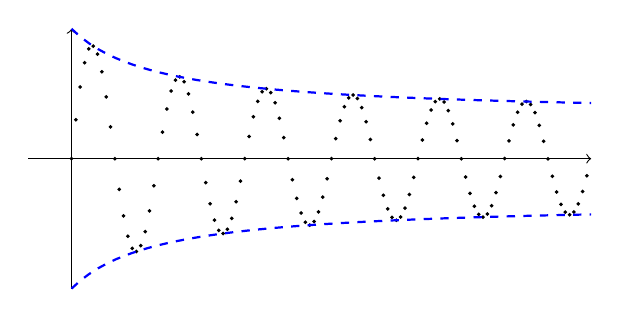
\begin{tikzpicture}[scale=1.1]
          \draw[->] (-0.5,0) -- (6,0);
          \draw[->] (0,-1.5) -- (0,1.5);
          
          % Draw the sine wave with smaller dots through exactly 5 periods
          \foreach \x in {0, 0.05, 0.1, ..., 6}
            \filldraw[black] (\x, {((1/(\x+1))+0.5)*sin(2*pi*\x r)}) circle (0.4pt); 

          \draw[blue, dashed, thick] plot[domain=0:6, samples=60] (\x, {1/(\x+1)+0.5});
          \draw[blue, dashed, thick] plot[domain=0:6, samples=60] (\x, {-1/(\x+1)-0.5});
        \end{tikzpicture}
        \caption{In order to find the limsup, we first look the whole sequence in $\mathbb{N}$ and find the supremum. We now "decrease" our domain from $\mathbb{N}$ to $\{2, \ldots\}$, then $\{3, \ldots\}$, then $\{4, \ldots\}$ and so on, continuing to label the supremum of the sequence. The limit of this sequence of supremums is the limsup.}
        \label{fig:limsupinf1}
      \end{subfigure}
      \hfill 
      \begin{subfigure}[b]{0.48\textwidth}
        \centering
        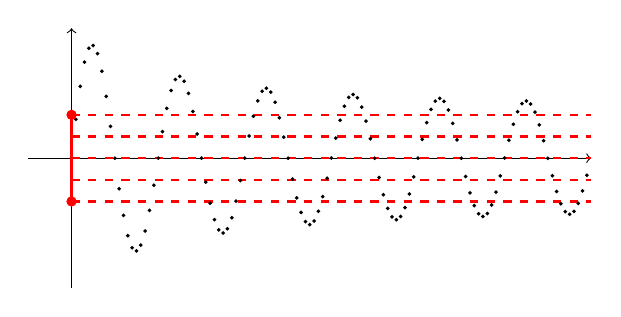
\begin{tikzpicture}[scale=1.1]
          \draw[->] (-0.5,0) -- (6,0);
          \draw[->] (0,-1.5) -- (0,1.5);
          \draw[-, red, dashed, thick] (0,0.5) -- (6,0.5);
          \draw[-, red, dashed, thick] (0,0.25) -- (6,0.25);
          \draw[-, red, dashed, thick] (0,0) -- (6,0);
          \draw[-, red, dashed, thick] (0,-0.25) -- (6,-0.25);
          \draw[-, red, dashed, thick] (0,-0.5) -- (6,-0.5);
          
          % Draw the sine wave with smaller dots through exactly 5 periods
          \foreach \x in {0, 0.05, 0.1, ..., 6}
            \filldraw[black] (\x, {((1/(\x+1))+0.5)*sin(2*pi*\x r)}) circle (0.4pt); 

          \draw[red, very thick] (0,-0.5) -- (0,0.5);
          \filldraw[red] (0,-0.5) circle (1.5pt);
          \filldraw[red] (0,0.5) circle (1.5pt);
        \end{tikzpicture}
        \caption{The 5 red lines marked in the middle (along with infinitely many others) are viable partial limits because one can choose a subsequence such that all of its points after a certain $n$ lie in some $\epsilon$-neighborhood of the limit. Therefore, we claim that the limsup/inf is the supremum of this set $E$.}
        \label{fig:limsupinf2}
      \end{subfigure}
      \caption{Two ways to visualize the superior and inferior limits of the divergent sequence $x_n = \big(\frac{1}{x+1} + 0.5\big) \sin(2\pi x)$. The left is the limit of the supremum, and the right is the supremum of the closed set of subsequential limits.} 
      \label{fig:limsupinf}
    \end{figure}
  \end{definition}

  \begin{example}[Computing Limsup and Liminf]
    We give some basic examples. 
    \begin{enumerate}
      \item Let $x_n = (-1)^n$. Then $E = \{-1, +1\}$ and 
      \begin{equation}
        \limsup_{n \rightarrow \infty} x_n = 1, \qquad \liminf_{n \rightarrow \infty} x_n = -1 
      \end{equation}

      \item Let $x_n = (-1)^n / [1 + (1/n)]$. Then 
      \begin{equation}
        \limsup_{n \rightarrow \infty} x_n = 1, \qquad \liminf_{n \rightarrow \infty} x_n = -1
      \end{equation}
    \end{enumerate}
  \end{example}

  Let's give two warnings. First, limsup and liminfs do \textit{not} behave like limits under addition and multiplication. That is, 
  \begin{equation}
    \limsup x_n + \limsup y_n \neq \limsup x_n + y_n 
  \end{equation}

  \begin{example}[Counterexamples of Arithmetic Consistency of Limit superior]
    Consider $(x_n) = (-1)^n$ and $y_n = (-1)^{n+1}$. Then 
    \begin{equation}
      \limsup x_n = \limsup y_n = 1, \qquad \liminf x_n = \liminf y_n = -1
    \end{equation}
    But $(x_n + y_n) = 0$, so 
    \begin{equation}
      \limsup x_n + y_n = \liminf x_n + y_n = 0 
    \end{equation}
  \end{example}

  Second, note that even though we are talking about subsequential limits, the limsup and liminf are \textit{not} subsequential limits! It is the supremum of subsequential limits $E$, which may or may not be in $E$. 

  \begin{example}[Limsup that is not attained by any subsequential limit]
    This should be a sequence not in $\mathbb{R}$. 
  \end{example}

  However, in $\mathbb{R}$, it turns out that the limsup and liminf are both contained in $E$, so we are fine. 

  \begin{lemma} 
    If $(x_n)$ is a sequence in $\mathbb{R}$, then 
    \begin{enumerate}
      \item the limsup is indeed a subsequential limit, i.e. $\limsup x_n \in E$. 
      \item If $x > \limsup x_n$, then $\exists N \in \mathbb{N}$ s.t. $n \geq N \implies x_n < x$. 
    \end{enumerate}
  \end{lemma}
  \begin{proof}
    For the first claim, there are two cases to consider. If $(x_n)$ is unbounded from above, then $\exists (x_{n_k})$ such that $x_{n_k} \rightarrow +\infty \implies \infty = \limsup x_n \in E$. If $(x_n)$ is bounded from above, then the subsequential limits of $(x_n)$ are either in $(x_n)$ or they are limit points of $x_n$. This implies that the set $E$ consists of points either in $\{x_n\}$ or are limit points of the set $\{x_n\} \implies \sup{E}$ is in $E$ since it's a limit point. 

    For the second claim, if there are infinitely many terms of the sequence larger than $x$, then we could find a subsequence $(x_{n_k})$ with $x_{n_k} > x$ for all $k$. Therefore $(x_n)$ has a subsequential limit which must be $\geq x$. Every subsequential limit of $(x_{n_k})$ is also a subsequential limit of $(x_n)$. This contradicts $\limsup x_n = \sup E$. 
  \end{proof}

  \begin{theorem}[Requirements of Partial Limits for Limit to Exist]
    Here are two results in which we can use partial limits to determine if a sequence has a limit or not. 
    \begin{enumerate}
      \item A sequence has a limit or tends to $\pm \infty$ if and only if its inferior and superior limits are the same. 
      \begin{equation}
        \limsup x_n = \liminf x_n = x \implies \lim_{n \rightarrow +\infty} x_n = x
      \end{equation}
      \item A sequence converges if and only if every subsequence of it converges. 
    \end{enumerate}
  \end{theorem}
  \begin{proof}
    For (1), we pick $x + \epsilon > x$. Then every term past some $N_1$ must be less than $x + \epsilon$. By the same logic, we have $N_2$ for $x - \epsilon < x$. So take $N = \max\{N_1, N_2\}$, which is contained in the $\epsilon$-ball around $x$. 
  \end{proof}

  \begin{theorem}[Ordering on Subsequential Limits]
    If $s_n \leq t_n$ for $n \geq N$, where $N$ is fixed, then 
    \begin{align*}
      \liminf_{n \rightarrow \infty} s_n & \leq \liminf_{n \rightarrow \infty} t_n \\
      \limsup_{n \rightarrow \infty} s_n & \leq \liminf_{n \rightarrow \infty} t_n 
    \end{align*}
  \end{theorem} 

  \begin{example}
    We claim 
    \begin{equation}
      \lim_{n \rightarrow \infty} n^{1/n} = 1 
    \end{equation}
    We can consider $x_n = n^{1/n} - 1$ and want to show that $x_n \rightarrow 0$. We have $x_n \geq 0$. If $n > 1$, then $n = (x_n + 1)^n \geq x_n^2 \cdot \frac{n(n - 1)}{2}$ from the binomial theorem. This means that 
    \begin{equation}
      x_n^2 \leq \frac{2}{n-1} \implies 0 \leq x_n \leq \sqrt{\frac{2}{n-1}} \rightarrow 0
    \end{equation}
    And so by the squeeze theorem, $x_n \rightarrow 0$. 
  \end{example}

  \begin{example}
    If $x > 1, \alpha \in \mathbb{R}$, then 
    \begin{equation}
      \lim_{n \rightarrow +\infty} \frac{n^\alpha}{x^n} = 0
    \end{equation} 
  \end{example}
 
\subsection{Convergence Tests for Real Series}

  \begin{definition}[Series over $\mathbb{R}$]
    Given a sequence of real numbers $(x_n)$, the \textbf{series (of partial sums)} is the sequence 
    \begin{equation}
      (s_n) = \sum_{k=1}^n x_k
    \end{equation}
    The \textbf{sum of the series} is the limit of $(s_n)$. Usually we define $(s_n)$ implicitly and use the summation notation. 
    \begin{equation}
      \sum_{n=1}^\infty x_n \coloneqq \lim_{n \rightarrow \infty} s_n
    \end{equation}
    \begin{enumerate}
      \item If the sequence $(s_n)$ converges to $s$, the series is \textbf{convergent}, written 
      \begin{equation}
        \sum x_n < +\infty
      \end{equation}
      \item If the sequence does not converge, it is \textbf{divergent}. 
      \item If the series of partial sums of $(|x_n|)$ converges, then it is said to be \textbf{absolutely convergent}.\footnote{Clearly, every absolutely convergent series is convergent because $\big|\sum_{n=1}^\infty a_n \big| \leq \sum_{n=1}^\infty |a_n|$. This is sort of the infinite analogue of the triangle inequality.}
      \begin{equation}
        \sum_{n=1}^\infty |x_n|
      \end{equation}
    \end{enumerate}
  \end{definition}

  We must reiterate a few warnings here. Note that the series $\sum x_n$ is simply notation and should \textit{not} be treated as an ``infinite sum.'' Such a thing does not exist for algebraic structures which have finary operations. More specifically, given a series, we cannot in general split nor combine series, and we cannot reindex nor rearrange (an infinite number of) terms. However, we can manipulate each term for a fixed index. 

  \begin{example}[Disasters of Reindexing and Rearranging]
    Let us take the series $\sum 0$. We clearly know that the corresponding sequence of partial sums $0, 0, \ldots$ is convergent to $0$. But if we do this series of steps. 
    \begin{align}
      \sum_{n=1}^\infty 0 & = \sum_{n=1}^\infty n - n && \tag{Can manipulate terms} \\
                          & = \sum_{n=1}^\infty n - \sum_{n=1}^\infty n && \tag{Cannot split series} \\ 
                          & = 1 + \sum_{n=2}^\infty n - \sum_{n=1}^\infty n && \tag{Can take 1st term out} \\ 
                          & = 1 + \sum_{n=1}^\infty (n+1) - \sum_{n=1}^\infty n && \tag{Cannot reindexing} \\
                          & = 1 + \sum_{n=1}^\infty (n+1) - n  && \tag{Cannot combine series} \\
                          & = 1 + \sum_{n=1}^\infty 1 && \tag{Can manipulate terms} \\
                          & = 1 + \infty = +\infty
    \end{align}
    The wrong steps show that the series is divergent. 
  \end{example} 

  We have seen the consequences of these mistakes that beginners make and are often on popular media. However, note that we can always do splitting, combining, reindexing, and rearranging for \textit{finite sums}, which are algebraically defined. Later on, we will show that some of these operations are allows for series that we know are convergent. 

  \begin{lemma}[All Series in Extended Positive Reals Converge]
    All series in $\mathbb{R}_{\geq 0} \cup \{+\infty\}$ converge. 
    \begin{equation}
      \sum_{n=1}^\infty x_n \in [0, +\infty]
    \end{equation}
  \end{lemma}
  \begin{proof}
    
  \end{proof}

  Since the convergence of a series is equivalent to convergence of its sequence of partial sums, applying the Cauchy convergence criterion to the sequence $\{s_n\}$ leads to the following theorem. 

  \begin{theorem}[Cauchy Convergence Criterion for Series]
    The series $a_1 + \ldots + a_n + \ldots$ converges if and only if for every $\epsilon > 0$ there exists $N \in \mathbb{N}$ such that for all $m \geq n > N$, 
    \begin{equation}
      |a_n + \ldots + a_m| < \epsilon
    \end{equation}
  \end{theorem}

  \begin{corollary}[nth Term Test]
    A necessary (but not sufficient) condition for convergence of the series $a_1 + \ldots a_n + \ldots$ is that the terms tend to $0$ as $n \rightarrow \infty$. That is, it is necessary that
    \begin{equation}
      \lim_{n\rightarrow \infty} a_n = 0
    \end{equation}
  \end{corollary}
  \begin{proof}
    It suffices to set $m = n$ in the Cauchy convergence criterion. This would mean that for every $\epsilon > 0$ there exists a $N \in \mathbb{N}$ such that 
    \begin{equation}
      |a_n| = |a_n - 0| < \epsilon \text{ for all } n > N
    \end{equation}
    which, by definition, means that $\{a_n\}$ converges to $0$. 
  \end{proof} 

  Nothing so far is really suprising here. The Cauchy convergence criterion really just follows from the definition of Cauchy completeness, and the $n$th term test is pretty trivial. The way that we will build up convergence tests is by proving some special cases of convergence and then using the direct comparison test to then classify further series.     

  \begin{example}[Telescoping Series]
    A \textbf{telescoping series} is a series in which the partial sums can cancel out. An example is the series of partial sums of the sequence $(x_n) = \frac{1}{n (n+1)}$. In here, the series term is
    \begin{align}
      s_n & = \sum_{k=1}^n \frac{1}{k(k+1)} \\ 
          & = \sum_{k=1}^n \frac{1}{k} - \frac{1}{k+1} \\
          & = \sum_{k=1}^n \frac{1}{k} - \sum_{k=1}^n \frac{1}{k+1} \\
          & = \sum_{k=1}^n \frac{1}{k} - \sum_{k=2}^{n+1} \frac{1}{k} \\
          & = \frac{1}{1} + \bigg( \sum_{k=2}^n \frac{1}{k} \bigg) - \bigg( \sum_{k=2}^n \frac{1}{k} \bigg) - \frac{1}{n+1} \\
          & = 1 + \bigg( \sum_{k=2}^n \frac{1}{k} - \frac{1}{k} \bigg) - \frac{1}{n+1} \\
          & = 1 - \bigg( \sum_{k=2}^n 0 \bigg) - \frac{1}{n+1} \\
          & = 1 - \frac{1}{n+1} 
    \end{align} 
    Note that all of the examples that we have done here are for finite sums, so they are all legal. 
  \end{example}

  \begin{example}[Geometric Series]
    The series $\sum_{n=0}^\infty q^n$ is called a \textbf{geometric series}. 
    \begin{equation}
      1 + q + q^2 + \ldots + q^n + \ldots
    \end{equation}
    is called the \textbf{geometric series}. We can see that 
    \begin{enumerate}
      \item $|q| \geq 1 \iff \sum q^n$ is divergent. $|q| \geq 1 \implies |q|^n \geq 1$, and so the terms $q^n$ does not converge to $0$, and the $n$th term test is not met. 
      \item $|q| < 1 \iff \sum q^n$ is convergent. We can use the identity 
      \begin{equation}
        s_n = 1 + q + \ldots + q^{n-1} = \frac{1 - q^n}{1-q} \implies \lim_{n \rightarrow \infty} \frac{1 - q^n}{1 - q} = \frac{1}{1 - q}
      \end{equation} 
      since $\lim_{n\rightarrow \infty} q^n = 0$ if $|q|<1$. 
    \end{enumerate}
  \end{example}

  The Cauchy convergence criterion can be used to prove the direct comparison test. 

  \begin{theorem}[Direct Comparison Test] 
    For some fixed $N$, if 
    \begin{enumerate}
      \item If $|x_n| \leq y_n$ for all $n \geq N$ and $\sum y_n$ converges, then $\sum x_n$ converges. 
      \item If $x_n \geq y_n \geq 0$ for all $n \geq N$  and $\sum y_n$ diverges, then $\sum x_n$ diverges. 
    \end{enumerate}
  \end{theorem} 

  \begin{example}[Comparison with Telescoping Series]
    We can prove the special case a geometric series with the direct comparison test. We claim that $\sum_{n=1}^\infty \frac{1}{n^2}$ is finite. We can see that 
    \begin{equation}
      \frac{1}{n^2} \leq \frac{2}{n (n+1)} 
    \end{equation}
    where the series of the terms in the RHS is telescoping and therefore converges. So by the direct comparison test, $\sum \frac{1}{n^2}$ converges. 
  \end{example}

  Now we prove another corollary of the Cauchy convergence criterion.   

  \begin{theorem}[Cauchy Condensation Test]
    If $a_1 \geq a_2 \geq \ldots \geq 0$, the series $\sum_{n=1}^\infty a_n$ converges if and only if the series 
    \begin{equation}
      \sum_{k=0}^\infty 2^k a_{2^k} = a_1 + 2 a_2 + 4a_4 + 8a_8 + \ldots 
    \end{equation}
    converges. 
  \end{theorem}
  \begin{proof}
    Letting $A_k = a_1 + a_2 + \ldots + a_k$ and $S_n = a_1 + 2a_2 + \ldots + 2^n a_{2^n}$, it is clear that by adding up the inequalities
    \begin{align*}
      & a_2 \leq a_2 \leq a_1 \\
      & 2a_4 \leq a_3 + a_4 \leq 2a_2 \\
      & 4a_8 \leq a_5 + a_6 + a_7 + a_8 \leq 4a_4 \\
      & \ldots \\
      & 2^n a_{2^{n+1}} \leq a_{2^n + 1} + \ldots + a_{2^{n+1}} \leq 2^n a_{2^n}, 
    \end{align*}
    we get
    \begin{equation}
      \frac{1}{2}(S_{n+1} - a_1) \leq A_{2^{n+1}} - a_1 \leq S_n
    \end{equation}
    Since the sequences $\{A_k\}$ and $\{S_k\}$ are nondecreasing, and hence from the inequalities we can conclude that they are either both bounded above (which means that they are both convergent since it is a bounded, nondecreasing series) or both unbounded above (which means that they are both divergent since they are nondecreasing and unbounded). 
  \end{proof}

  \begin{corollary}[p-series Test]
    The series 
    \begin{equation}
      \sum_{n=1}^\infty \frac{1}{n^p}
    \end{equation}
    converges for $p>1$ and diverges for $p \leq 1$.\footnote{This sort of reminds you of $u$-substitution. For example, look at $\int_1^\infty f(t) \,dt = \int_0^\infty e^u f(e^u)\,du$, where the convergence of LHS $\iff$ convergence of RHS.}
  \end{corollary}
  \begin{proof}
    Suppose $p\geq 0$. By the previous theorem, the series converges or diverges simultaneously with the series 
    \begin{equation}
      \sum_{k=0}^\infty 2^k \frac{1}{(2^k)^p} = \sum_{k=0}^\infty (2^{1-p})^k
    \end{equation}
    which is really just a geometric series. A necessary and sufficient condition for the convergence of this series is that $2^{1-p} < 1$, that is, $p>1$. 

    Now suppose $p \leq 0$. The series is then clearly divergent since all of the terms are larger than $1$. 
  \end{proof}

  \begin{example}[Harmonic Series]
    The \textbf{harmonic series} 
    \begin{equation}
      1 + \frac{1}{2} + \frac{1}{3} + \ldots + \frac{1}{n} + \ldots
    \end{equation}
    seems at first glance to be converging since the terms converge to $0$. However, it does not pass the Cauchy condensation test since 
    \begin{equation}
      \sum_{n=1}^\infty 2^n x_n = \sum_{n=1}^\infty 2^n \frac{1}{2^n} = \sum_{n=1}^\infty 1 = +\infty
    \end{equation}
    As you can see, this increases logarithmically, so in early calculators it was hard to numerically detect divergence (you would have to double the number of series terms to get a linear increase). 
  \end{example} 

\subsection{Ratio and Root Tests} 

  Now we introduce the root and ratio tests, which are derived by the comparison test with a geometric series. The ratio test is used more day-to-day, but not as decisive as the root test. Both tests have a similar flavor. 

  \begin{theorem}[Ratio Test]
    Suppose the limit $\lim_{n\rightarrow \infty} \big| \frac{a_{n+1}}{a_n} \big| = \alpha$ exists for the series $\sum_{n=1}^\infty a_n$. Then, 
    \begin{enumerate}
      \item $\alpha < 1 \implies \sum a_n$ converges absolutely. 
      \item $\alpha > 1 \implies \sum a_n$ diverges.
      \item $\alpha = 1 \implies \sum a_n$ is inconclusive. 
    \end{enumerate}
    Alternatively, if 
    \begin{enumerate}
      \item $\limsup |a_{n+1}/a_n| = \alpha < 1$, then $\sum a_n$ converges 
      \item If $\exists N$ s.t. $|a_{n+1}/a_n| \geq 1$ for all $n \geq N$, then $\sum a_n$ diverges. 
    \end{enumerate}
  \end{theorem}
  \begin{proof}
    Since $\limsup \big| \frac{a_{n+1}}{a_n} \big| = \alpha < 1$, fix any $\alpha < \beta < 1$. Then $\exists N$ s.t. if $n > N$, $|a_{n+1}/a_n| < \beta$. So $|a_{N+1}| < \beta |a_N| \implies |a_{N+2}| < \beta^2 |a_N|$. So letting $C = |a_N|$, for all $m \geq N$, 
    \begin{equation}
      |a_m| \leq \frac{C}{\beta^N} \beta^m \implies |a_m| \leq \Tilde{C} \beta^m \text{ for all } m \geq N
    \end{equation}
    So $\sum a_n$ converges by comparison test since $\sum \beta^m < \infty$ when $\beta < 1$. 
  \end{proof}

  \begin{theorem}[Root Test]
    Let $\sum_{n=1}^\infty a_n$ be a given series and 
    \begin{equation}
      \alpha = \limsup_{n\rightarrow \infty} \sqrt[n]{|a_n|}
    \end{equation}
    Then, 
    \begin{enumerate}
      \item $\alpha < 1 \implies \sum a_n$ converges. 
      \item $\alpha > 1 \implies \sum a_n$ diverges. 
      \item $\alpha = 1 \implies \sum a_n$ is inconclusive. 
    \end{enumerate}
  \end{theorem} 
  \begin{proof}
    Listed. 
    \begin{enumerate}
      \item If $\limsup \sqrt[n]{|a_n|} = \alpha < 1$, take any $\alpha < \beta < 1$. Then $\exists N \in \mathbb{N}$ s.t. if $n \geq N$, then $|a_n|^{1/n} < \beta \iff |a_n| < \beta^n$. Since $\beta < 1$, $\sum \beta^n < \infty$, and by comparison test, $\sum a_n$ converges. 

      \item Suppose $\alpha > 1$. Then $\limsup |a_n|^{1/n} = \alpha > 1$. So there exists a subsequence $(a_{n_k})$ s.t. $(|a_{n_k}|^{1/n_k}) \rightarrow \alpha > 1$. This means $\exists N$ s.t. for $n \geq N$, $|a_{n_k}|^{1/{n_k}} > 1 \implies |a_{n_k}| > 1$. But this fails the $n$th term test. 

      \item We do not claim anything and so there's nothing to prove. 
    \end{enumerate}
  \end{proof}

  \begin{example}[Root Test Inconclusive Results]
    Consider $\sum \frac{1}{n} = +\infty$, but from the root test 
    \begin{equation}
      \sqrt[n]{\frac{1}{n}} \rightarrow 1, \text{ so } \alpha = 1
    \end{equation}
    Consider $\sum \frac{1}{n^2} < +\infty$, but from from the root test 
    \begin{equation}
      \sqrt[n]{\frac{1}{n^2}} = \bigg( \frac{1}{n^{1/n}} \bigg)^2 \rightarrow 1, \text{ so } \alpha = 1
    \end{equation}
  \end{example}

  \begin{example}
    The sequence $\sum \frac{c^n}{n!}$ always converges for $c \in \mathbb{R}$. 
  \end{example}

  \begin{theorem}[Weierstrass M-test for Absolute Convergence]
    Let $\sum_{n=1}^\infty a_n$ and $\sum_{n=1}^\infty b_n$ be series. Suppose there exists an index $N \in \mathbb{N}$ such that $|a_n| \leq b_n$ for all $n>N$. Then, 
    \begin{equation}
      \sum_{n=1}^\infty b_n \text{ converges } \implies \sum_{n=1}^\infty a_n \text{ converges absolutely}
    \end{equation}
  \end{theorem}

  We finally conclude by giving a theorem about the convergence of some special sequences. 

  \begin{theorem}[Special Sequences]
    Some special sequences: 
    \begin{enumerate}
      \item If $p > 0$, then $\lim_{n \rightarrow \infty} \frac{1}{n^p} = 0$. 
      
      \item If $p > 0$, then $\lim_{n \rightarrow \infty} \sqrt[n]{p} = 1$. 

      \item $\lim_{n \rightarrow \infty} \sqrt[n]{n} = 1$. 

      \item If $p > 0$ and $\alpha$ is real, then $\lim_{n \rightarrow \infty} \frac{n^\alpha}{(1 + p)^n} = 0$. 
      
      \item If $|x| < 1$, then $\lim_{n \rightarrow \infty} x^n = 0$. 
    \end{enumerate}
  \end{theorem}

\subsection{Euler's Number and Trigonometric Functions} 

  \begin{definition}[Euler's Number]
    We define \textbf{Euler's number} as 
    \begin{equation}
      e \coloneqq \sum_{n=0}^\infty \frac{1}{n!}
    \end{equation}
  \end{definition}
  
  The first thing we should do is show that it converges, this is a one-liner. 
  \begin{equation}
    \sum_{n=0}^\infty \frac{1}{n!} = 1 + 1 + \sum_{n=2}^\infty \frac{1}{n!} \leq 2 + \sum_{n=2}^\infty \frac{1}{n(n-1)} 
  \end{equation}

  \begin{theorem}[Euler's Number as a Limit]
    We have 
    \begin{equation}
      \lim_{n \rightarrow +\infty} \bigg( 1 + \frac{1}{n} \bigg)^n = e 
    \end{equation}
  \end{theorem}
  \begin{proof}
    Let us define the sequence 
    \begin{equation}
      t_n = \sum_{k=0}^n \frac{1}{k!}, \qquad s_n = \bigg( 1 + \frac{1}{n} \bigg)^n
    \end{equation}
    We know that $t_n \rightarrow e$, and we want to show that $s_n \rightarrow e$. We do this with the squeeze theorem. 
    \begin{enumerate}
      \item We can see that 
      \begin{align}
        s_n & = \bigg( 1 + \frac{1}{n} \bigg)^n \\ 
            & = \sum_{k=0}^n \binom{n}{k} 1^{n-k} \bigg( \frac{1}{n} \bigg)^k \\
            & = 1 + 1 + \frac{n(n-1)}{2!} \frac{1}{n^2} + \frac{n(n-1)(n-2)}{3!} \frac{1}{n^3} + \ldots \\ 
            & = 1 + 1 + \frac{1}{2!} (1) \bigg( 1 - \frac{1}{n} \bigg) + \frac{1}{3!} (1) \bigg(1 - \frac{1}{n} \bigg) \bigg(1 - \frac{2}{n} \bigg) + \ldots + \frac{1}{n!} (1) \prod_{k=1}^{n-1} \bigg(1 - \frac{k}{n} \bigg) \\
            & \leq \frac{1}{0!} + \frac{1}{1!} + \frac{1}{2!} + \frac{1}{3!} + \ldots + \frac{1}{n!} = t_n 
      \end{align}
      and so $s_n < t_n \implies \limsup s_n \leq \limsup t_n = e$. 

      \item Let $m \leq n$ be fixed. Then, 
      \begin{equation}
        s_n \geq 1 + 1 + \frac{1}{2!} \bigg( 1 - \frac{1}{n} \bigg) + \ldots + \frac{1}{m!} \bigg(1 - \frac{1}{n} \bigg) \bigg(1 - \frac{2}{n} \bigg) \ldots \bigg(1 - \frac{m-1}{n} \bigg) 
      \end{equation}
      since we are just taking the first $m$ positive terms of the element. Therefore, letting $n \rightarrow +\infty$ and keeping $m$ fixed, we get 
      \begin{equation}
        \liminf_{n \rightarrow +\infty} s_n \geq 1 + 1 + \frac{1}{2!} + \ldots + \frac{1}{n!} \text{ for all } m \in \mathbb{N}
      \end{equation}
      which implies $\liminf s_n \geq t_m$ for all $m \in \mathbb{N}$, and now letting $m \rightarrow +\infty$, we have $\liminf s_n \geq \liminf t_m = e$. 
    \end{enumerate}
  \end{proof}

  Now we prove the irrationality of $e$. It is usually extremely difficult to prove that an arbitrary number is irrational, e.g. $\pi^e$ or $\pi^{e^e}$. 

  \begin{theorem}[$e$ is Irrational]
    $e$ is irrational. 
  \end{theorem}
  \begin{proof} 
    Letting $t_n = \sum_{k=0}^n \frac{1}{k!}$, we have 
    \begin{align}
      e - t_n & = \sum_{k=n+1}^\infty \frac{1}{k!} \\
              & = \frac{1}{(n+1)!} \bigg( 1 + \frac{1}{n+2} + \frac{1}{(n+3)(n+2)} + \ldots \bigg) \\
              & < \frac{1}{(n+1)!} \underbrace{\bigg( 1 + \frac{1}{n+2} + \frac{1}{(n+2)^2} + \ldots \bigg)}_{\text{geometric}} \\
              & = \frac{1}{(n+1)!} \bigg( \frac{1}{1 - (1/(n+2)!)}\bigg) \\
              & = \frac{1}{n! n} \cdot \underbrace{\frac{(n+2) n}{(n+1)^2}}_{< 1} \\
              & = \frac{1}{n! n}
    \end{align}
    Note that we can combine and split sums since we know that $e$ is convergent. Now suppose that $e = p/q$. Then, 
    \begin{equation}
      0 < q! (e - t_q) < \frac{1}{q}
    \end{equation}
    But $q! e$ is an integer and $q! t_q$ is also an integer. So we have $q! \cdot \frac{p}{q}$, an integer, between $0$ and $1$, which is a contradiction. 
  \end{proof}

  Since we have defined some number $e \in \mathbb{R}$, we know that exponential exist, and therefore we the function $x \mapsto e^x$ is well-defined. In fact, it is so important that we have a separate name for it. 

  \begin{definition}[Exponential Function]
    The \textbf{exponential function} is generally referred to as the function $x \mapsto e^x$. 
  \end{definition}

  There is a nice series representation. 

  \begin{theorem}[Exponential Function as a Series]
    We have 
    \begin{equation}
      e^x = \sum_{n=0}^\infty \frac{x^n}{n!}
    \end{equation}
  \end{theorem}
  \begin{proof}
    
  \end{proof}

  Now that this is done, we can define the trigonometric functions formally as such. 

  \begin{definition}[Trigonometric Functions]
    We have 
    \begin{align}
      \sin x&=\sum_{n=0}^{\infty}\frac{(-1)^n}{(2n+1)!}x^{2n+1}=x-\frac{x^3}{3!}+\frac{x^5}{5!}-\cdots
      \\\\
      \cos x&=\sum_{n=0}^{\infty}\frac{(-1)^n}{(2n)!}x^{2n}=1-\frac{x^2}{2!}+\frac{x^4}{4!}-\cdots
    \end{align}
  \end{definition}

